Multi-agent systems are essential in modern space operations. Distributed communication networks, GPS and imaging constellations, and rendezvous and docking procedures all rely on agents that must predict and coordinate with others to achieve mission success. Historically, these interactions have been treated as cooperative multi-agent problems, where all actors share a common objective. Such scenarios are typically solved as one-sided optimal control problems that determine the motion of all agents simultaneously. However, the rise of international competition has introduced an era of adversarial actors in the space domain. In this non-cooperative landscape, an agent must fulfill its own mission requirements, such as maintaining a specific orbital slot, while proactively mitigating risks posed by other agents with competing objectives.

Game theory provides a rigorous mathematical framework for navigating these strategic interactions. This approach treats pursuit-evasion as a two-sided optimization problem, seeking a Nash equilibrium: a state where neither agent can reduce their respective costs by unilaterally changing their control strategy. While these classical methods provide a theoretical foundation for optimal play, they often struggle with the nonlinear complexities and high dimensionality of orbital dynamics \cite{fu_analytical_2025} \cite{jia_approximate_2025}.
Another limitation is their reliance on deterministic, or ``pure," strategies. In a competitive environment, a deterministic strategy is inherently exploitable; if an opponent can predict a specific trajectory, they can utilize this information to counteract it \cite{peters2022learning}. Furthermore, existing literature frequently assumes the pursuer possesses superior fuel and agility, effectively guaranteeing capture \cite{venigalla2018spacecraft} \cite{pontani2009numerical}, though in practice this may not be true. 
% In reality, orbital constraints often lead to scenarios where no pure-strategy Nash equilibrium exists \red{CITE}. 

% \begin{figure}
%     \centering
%     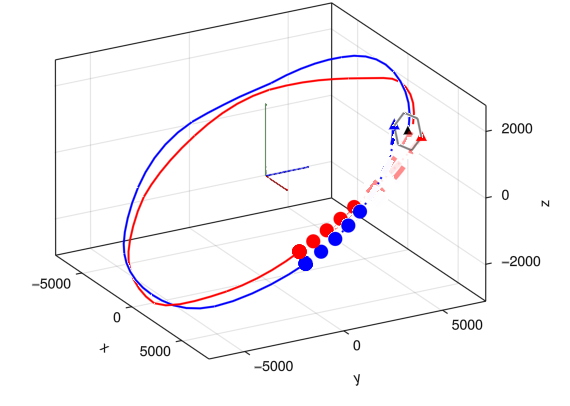
\includegraphics[width=\linewidth]{images/k_replan_10.png}
%     \caption{Game step }
%     \label{fig:placeholder}
% \end{figure}

Motivated from recent advances in robotics, we explore the use of mixed strategies, where players optimize over a finite set of candidate trajectories \cite{peters2022learning} \cite{hanlongResearchStrategiesMultiSpacecraft2024}, alleviating issues arising from deterministic play. 
% 
Additionally, by employing a framework for profiling agent behavior called fictitious play (FP), 
% 
% Additionally, by employing a framework for strategy-reasoning called fictitous play (FP), 
% 
agents can adapt to an opponent’s real-time actions \cite{albrechtReasoningHypotheticalAgent}. 
% 
In this work, we optimize over a discrete set of candidate trajectories to determine best-response strategies. Our primary contributions are as follows:

\begin{enumerate}
    \item We develop a methodology to project the continuous control pursuit-evasion game into a discrete set of candidate trajectories around a reference orbit.
    \item We utilize fictitious play, allowing an agent to profile an opponent's strategy in real-time.
    \item We provide a Monte Carlo table of stationary results by pitting various strategy types against one another: Greedy, Mixed, Random, and Fictitious Play.
\end{enumerate}

% 
% \begin{figure}[t!]
%     \centering
%     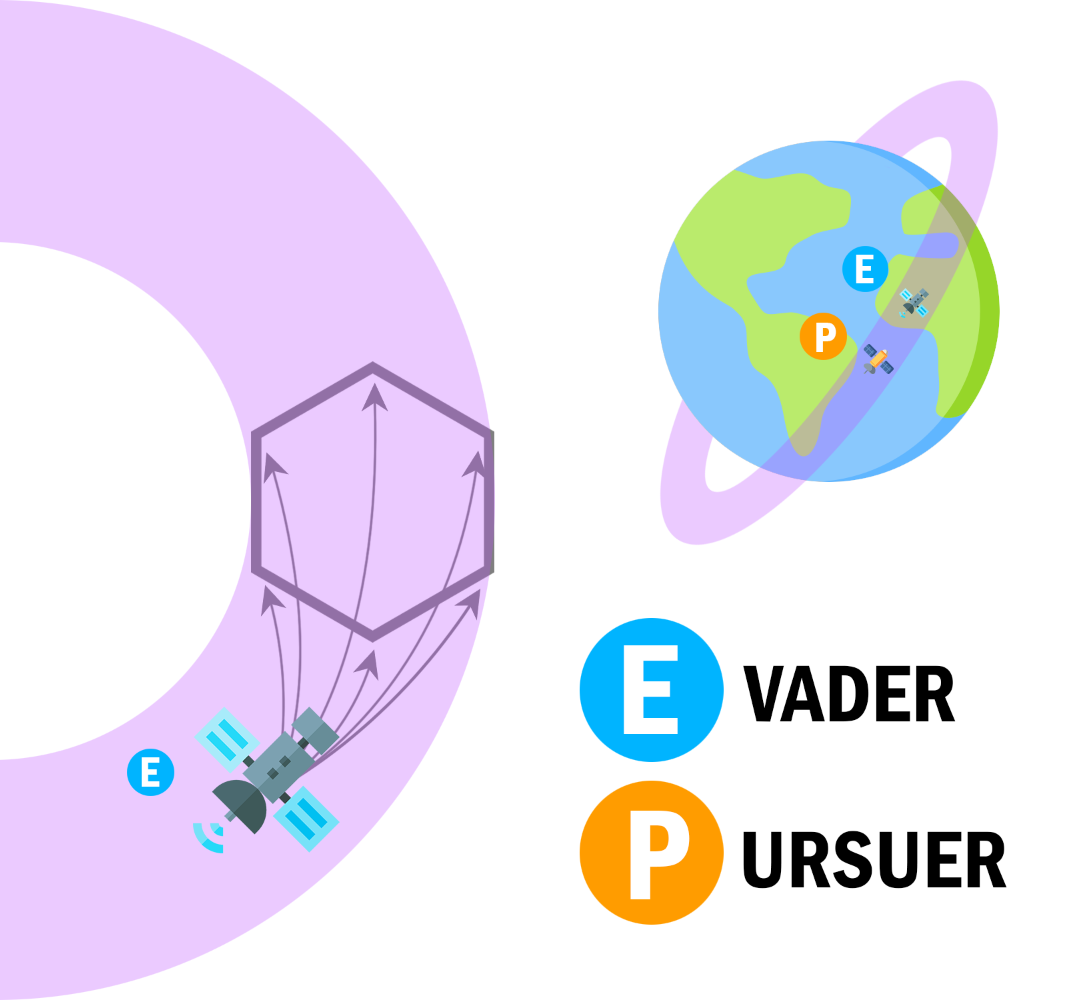
\includegraphics[width=0.5\textwidth]{images/evader_pursuer_diagram.png}
%     \caption{Evader-Pursuer diagram}
%     \label{fig:evader_pursuer_diagram}
% \end{figure}
% 

% The remainder of this paper is organized as follows: Section II reviews related work in orbital pursuit-evasion and mixed-strategy games; Section III formulates the orbital game and dynamics; Section IV details our approach to trajectory lifting and FP updates; Section V presents the results of our Monte Carlo simulations; and Section VI offers concluding remarks.